\documentclass[10pt,a4paper]{article}

\sloppy
\usepackage{caption}
\usepackage{subcaption}
\captionsetup[subfigure]{justification=centering}
\captionsetup{font = footnotesize, labelfont = bf}
\captionsetup[sub]{font=scriptsize,labelfont= bf, justification = centering, margin = 0cm}

\setlength{\textwidth}{16cm}
\setlength{\textheight}{23cm}
\addtolength{\hoffset}{-1.5cm}
\addtolength{\voffset}{-1.5cm}
\setlength{\headheight}{35pt}
\usepackage[utf8]{inputenc}
%\usepackage[spanish]{babel}
\usepackage[spanish,es-tabla]{babel}
\usepackage{ae}
\usepackage{graphicx}
\usepackage{wrapfig}
\usepackage{tikz,pgfplots}
\usepackage{epsfig}
%\usepackage{multicol, array}
\usepackage{amsmath}
\usepackage{amssymb, amsthm}
\usepackage{amsfonts}
\usepackage{mathtools}
\DeclareMathOperator\erf{erf}
\usepackage{euscript}
\usepackage{mathrsfs}
\usepackage{sectsty}
\usepackage{lipsum}
\usepackage{courier}
\usepackage{listings}
\usepackage{xcolor}
\definecolor{verde}{rgb}{0.0, 0.5, 0.1}

\lstset{
  language=R, literate =  {á}{{\'a}}1 {é}{{\'e}}1 {í}{{\'{\i}}}1 {ó}{{\'o}}1 {ú}{{\'u}}1 {Á}{{\'A}}1 {É}{{\'E}}1 {Í}{{\'I}}1 {Ó}{{\'O}}1 {Ú}{{\'U}}1 {ü}{{\"u}}1 {Ü}{{\"U}}1 {ñ}{{\~n}}1 {Ñ}{{\~N}}1,
  backgroundcolor=\color{gray!6!},
  classoffset=0,
  basicstyle=\ttfamily\small\bfseries,
  showspaces=false,
  showstringspaces=false,
  keywordstyle=\color{blue!60!black}\bfseries,
  stringstyle=\color{blue},
  numbers=none,
  numberstyle=\ttfamily\small,
  commentstyle=\color{verde}\textbf,
  morecomment=[l][\color{verde}\textbf],
  frame = single,
  framexleftmargin= -0pt,
  framexrightmargin= -5pt}


\usepackage{tcolorbox}
\tcbuselibrary{theorems}

\newtcbtheorem[auto counter,number within=section]{theorem}{Teorema}%
{colback=green!5,colframe=green!35!black,fonttitle=\bfseries}{th}

\newtcbtheorem[auto counter,number within=section]{definition}{Definición}%
{colback=blue!5,colframe=blue!35!black,fonttitle=\bfseries}{def}

\newtcbtheorem[auto counter,number within=section]{example}{Ejemplo}%
{colback=red!5,colframe=red!35!black,fonttitle=\bfseries}{ej}


%\newtcbtheorem[auto counter,number within=section]{theorem}{Teorema}%
%{colback=green!5,colframe=green!35!black,fonttitle=\bfseries}{th}

\newtcbtheorem[auto counter,number within=section]{software}{Software}%
{colback=yellow!5,colframe=yellow!35!black,fonttitle=\bfseries}{sw}

\usepackage{fancyhdr}

\decimalpoint
\usepackage[T1]{fontenc}
%\usepackage{textcomp}

\pagestyle{fancy}
\lhead{U.N.S.L. - Departamento de Física - 2021\\Lic. en Física - Mecánica del Continuo}
%\rhead{
\includegraphics[width=0.8cm]{/home/juan/Documentos/Docencia/unsl.jpg}}
%\pagenumbering{arabic}
\rhead{
\includegraphics[width=0.8cm]{/home/juan/Documentos/Docencia/unsl.jpg}}

%\setcounter{page}{1}
\setlength{\parskip}{3mm}

\pgfplotsset{compat=1.13}

\usepackage{hyperref}
\hypersetup{
    colorlinks=true,
    linkcolor=blue,
    filecolor=black,      
    urlcolor=blue,
    citecolor=black,
   	anchorcolor=black
}
 
\urlstyle{same}
\usepackage{lettrine}
\setcounter{DefaultLines}{4}
% \renewcommand{\tablename}{Tabla}
\begin{document}
\begin{center}
\bf{Mecánica del Continuo} \vspace*{0.2cm} \linebreak
\vspace{0.050cm}
\begin{Large}\bf{Consulta TP N 3} \end{Large} \vspace*{0.2cm}\\ \bf{Cinemática de medios poco discretos (más bien continuos)}
 \end{center}
\begin{center}
--------------------------------------------------------------------------------------------------
\end{center} 

\section*{Ejercicio 2}


Un cuerpo está rotando con una velocidad angular $\omega = \omega_1 \, e_1 + \omega_2 \, e_2 + \omega_3 \,e_3$.

\begin{itemize}
\item[\textbf{a)}] Encuentre el campo de velocidades asociado en coordenadas cartesianas.
\item[\textbf{b)}] Suponga $\omega = |\omega| e_3$. Evalúe las funciones que encontró en el punto (a).
\item[\textbf{c)}] Encuentre el campo de aceleración en coordenadas cartesianas para \linebreak $\omega = |\omega| \, e_3$.
\item[\textbf{d)}] ¿la velocidad de cada partícula varía en el tiempo? ¿cómo relaciona la aceleración con la pregunta anterior? 
\end{itemize}

\begin{center}------------------------------------------------------------------------------\end{center}

\subsection*{Solución}

\textbf{a)} Para encontrar el campo de velocidades asociado, sólo tenemos que saber que:

\begin{equation}\label{ecvxomega}
\mathbf{v} = \mathbf{\omega} \times \mathbf{x}
\end{equation}

\noindent donde esta ecuación no es tan familiar, sólo porque en todas las físicas teóricas se ven las cosas en un plano...pero basta con proponer esta ecuación en un caso simple y darle una vuelta para ver que no es nada desquiciada.

Si en la ec.\eqref{ecvxomega} tenemos que $\mathbf{\omega} =  \omega_1 \mathbf{e_1} + \omega_2 \mathbf{e_2} + \omega_3 \mathbf{e_3}$ y representamos un punto cualquiera por un vector posición $\mathbf{x} = x_1 \mathbf{e_1} + x_2 \mathbf{e_2} + x_3 \mathbf{e_3}$, entonces tenemos:

\begin{equation}\label{eca}
\mathbf{v} = (\omega_2 x_3 - \omega_3 x_2)\mathbf{e_1} + (\omega_3 x_1 - \omega_1 x_3) \mathbf{e_2} + (\omega_1 x_2 - \omega_2 x_1) \mathbf{e_3}
\end{equation}


\noindent con lo que está listo el campo de velocidades.

\medskip

\textbf{b)} Este punto sale directamente, reemplazando en la ec.\eqref{eca} $\mathbf{\omega} = \omega_3 \mathbf{e_3} = |\omega| \mathbf{e_3}$:

\begin{equation}\label{ecb}
\mathbf{v} = -|\omega| x_2 \mathbf{e_1} + |\omega| x_1 \mathbf{e_2} + 0 \mathbf{e_3}
\end{equation}

\medskip
\textbf{c)} Para obtener el campo de aceleración, simplemente usamos la ec. que está en el libro, reemplazando la ec.\eqref{ecb}

\begin{equation}\label{ecc}
\mathbf{a} = \frac{\partial \mathbf{v}}{\partial t} + (\nabla \mathbf{v})\mathbf{v} = \mathbf{0} +
\begin{pmatrix*}[r]
0 &  -|\omega| & 0 \\ 
|\omega| &  0 & 0 \\ 
0 &  0 & 0 \\ 
\end{pmatrix*}
\begin{pmatrix*}[r]
-|\omega| x_2  \\
|\omega| x_1 \\
0 \\
\end{pmatrix*}  =
-|\omega|^2 x_1 \mathbf{e_1} - |\omega|^2 x_2 \mathbf{e_2}  
\end{equation}

\noindent donde en la ec.\eqref{ecc} nos entrega una aceleración que siempre apunta perpendicularmente al eje $\mathbf{e_3}$.

\textbf{d)} Esta la dejamos para la interpretación personal de cada une...que no es menor.


\section*{Ejercicio 4}

Considere el campo de deformación dado por $x = X + AX$, siendo $A$ un tensor de componentes $A_{ii}$ independientes de $X_i$.
 
\begin{itemize}
\item[a)] Realice gráficas en la forma del punto $(2.d)$ para un elemento material de su elección y para el ángulo $\theta$ entre dos elementos materiales --también a su elección-- comparando con el tensor $E$. Utilice valores $0 < A_{ii} < 0.5$
\item[b)] Agregue a las gráficas anteriores un tensor $E^A = (A+A^T)/2$ y compare. ¿para qué rango de $A_{ii}$ la aproximación es válida?
\end{itemize}

\begin{center}------------------------------------------------------------------------------\end{center}

\subsection*{Solución Ej 4}

\textbf{a)} Tenemos que la deformación está dada por:

\begin{equation}\label{ed}
\mathbf{x} = \mathbf{X} + \mathbf{AX} = \mathbf{X} + k \mathbf{IX}
\end{equation}

\noindent donde el símbolo $\mathbf{I}$ es el tensor identidad.

De la ec.\eqref{ed}, podemos identificar el campo de deformación $\mathbf{u} = k \mathbf{X}$. Luego el tensor \textit{gradiente de deformación} como:

\begin{equation}\label{egdef}
\nabla u = 
\begin{pmatrix}
k &  0 & 0 \\ 
0 &  k & 0 \\ 
0 &  0 & k \\ 
\end{pmatrix}
\end{equation}

\noindent donde vemos que el tensor $\nabla u$ es simétrico.

Sabiendo el gradiente de deformación, es posible calcular, a partir de un elemento no deformado, $d\mathbf{X}$, el elemento deformado $d\mathbf{x}$, utilizando la ec. del libro de texto $d\mathbf{x} = d\mathbf{X} + \nabla \mathbf{u} d\mathbf{X}$.

Eligiendo dos elementos materiales inicialmente perpendiculares, $d\mathbf{X^{(1)}} = dS \mathbf{e_1}$ y $d\mathbf{X^{(2)}} = dS \mathbf{e_2}$, tenemos que se deforman como:

\begin{equation}\label{eed}
d\mathbf{x^{(1)}} = (1  + k) \, dS \mathbf{e_1}  \quad \quad d\mathbf{x^{(2)}} = (1  + k ) \, dS \mathbf{e_2}  
\end{equation}

\noindent donde, como era esperable, aumentan su longitud en un factor $(1+k)$ y no modifican el ángulo entre ellos (que continua siendo de $\pi/2$ después de la transformación). Una forma usual de caracterizar un cambio en la elongación de un elemento $d\mathbf{X}$ es utilizar la \textit{deformación unitaria}, que no es otra cosa que  $(ds - dS)/dS$, donde $ds$ es la longitud del elemento deformado. Para las ecs. \eqref{eed} tenemos:

\begin{equation}\label{eelu}
\frac{ds^{(1)}-dS^{(1)}}{dS^{(1)}} = k  \quad \quad \frac{ds^{(2)}-dS^{(2)}}{dS^{(2)}} = k  
\end{equation}

\noindent donde ya tenemos nuestro gráfico predilecto (sin hacerlo): la elongación unitaria es una recta de pendiente $k$ conn ordenada al origen $0$.

Por otra parte, el \textit{tensor de deformación lagrangiano} $\mathbf{E}^*$, está dado por $\mathbf{E}^* = \nabla \mathbf{u} + (\nabla \mathbf{u})^T + (\nabla \mathbf{u})^T \nabla \mathbf{u}$, y caracteriza las deformaciones (es necesario leer un poco). Si consideramos deformaciones infinitesimales, el \textit{tensor de deformación infinitesimal} $\mathbf{E} = 1/2 (\nabla \mathbf{u} + (\nabla \mathbf{u}^T))$ es simétrico, y descarta los términos de $O(>1)$ presentes en $\mathbf{E}^*$\footnote{En mecánica de medios continuos, sobre todo en la parte de sólidos, es usual que las deformaciones sean infinitesimales, dado que (a) Los regímenes donde valen los modelos presentan zonas de deformaciones permanentes si las deformaciones son grandes; (b) los esfuerzos aplicados tienen correlato con las deformaciones por medio de constantes que hacen que, aún con esfuerzos grandes, las deformaciones sean de una parte en $10^6$.}.

Si calculamos el tensor de deformación infinitesimal, tenemos:
\begin{equation}
\mathbf{E} =\frac{1}{2}\big( \nabla \mathbf{u} + (\nabla \mathbf{u}) ^T  \big) = 
\begin{pmatrix}
k &  0 & 0 \\ 
0 &  k & 0 \\ 
0 &  0 & k \\ 
\end{pmatrix}
\end{equation}

\noindent con lo que nuestro tensor de deformación infinitesimal $\mathbf{E}$ es igual al gradiente de deformación $\mathbf{u}$.

De cualquier forma, se lee en la ec. \textbf{3.8.1} que $ds^2 = dS^2 + 2dS^2 E_{nn}$ (sin suma en $n$). Dado que nuestro etnsor $\mathbf{E}$ tiene una diagonal $k$...¿cómo conciliar resultados?


Bueno, no termino de resolver porque la teoría \textit{merece una leída}.

Saludos cordiales, cualquier cosa me avisan.




%

%\begin{lstlisting}[language = Mathematica]
%StreamDensityPlot[{{1, 0}, -x}, {x, -5, 5}, {y, -5, 5}, 
% ColorFunction -> "RedBlueTones", StreamStyle -> Black, 
% StreamPoints -> Medium, ImageSize -> Large,
% PlotLabel -> "Campo de velocidades", 
% LabelStyle -> Directive[Bold, Orange]]
%
%\end{lstlisting}
%
%\begin{figure}[h!]
%\centering
%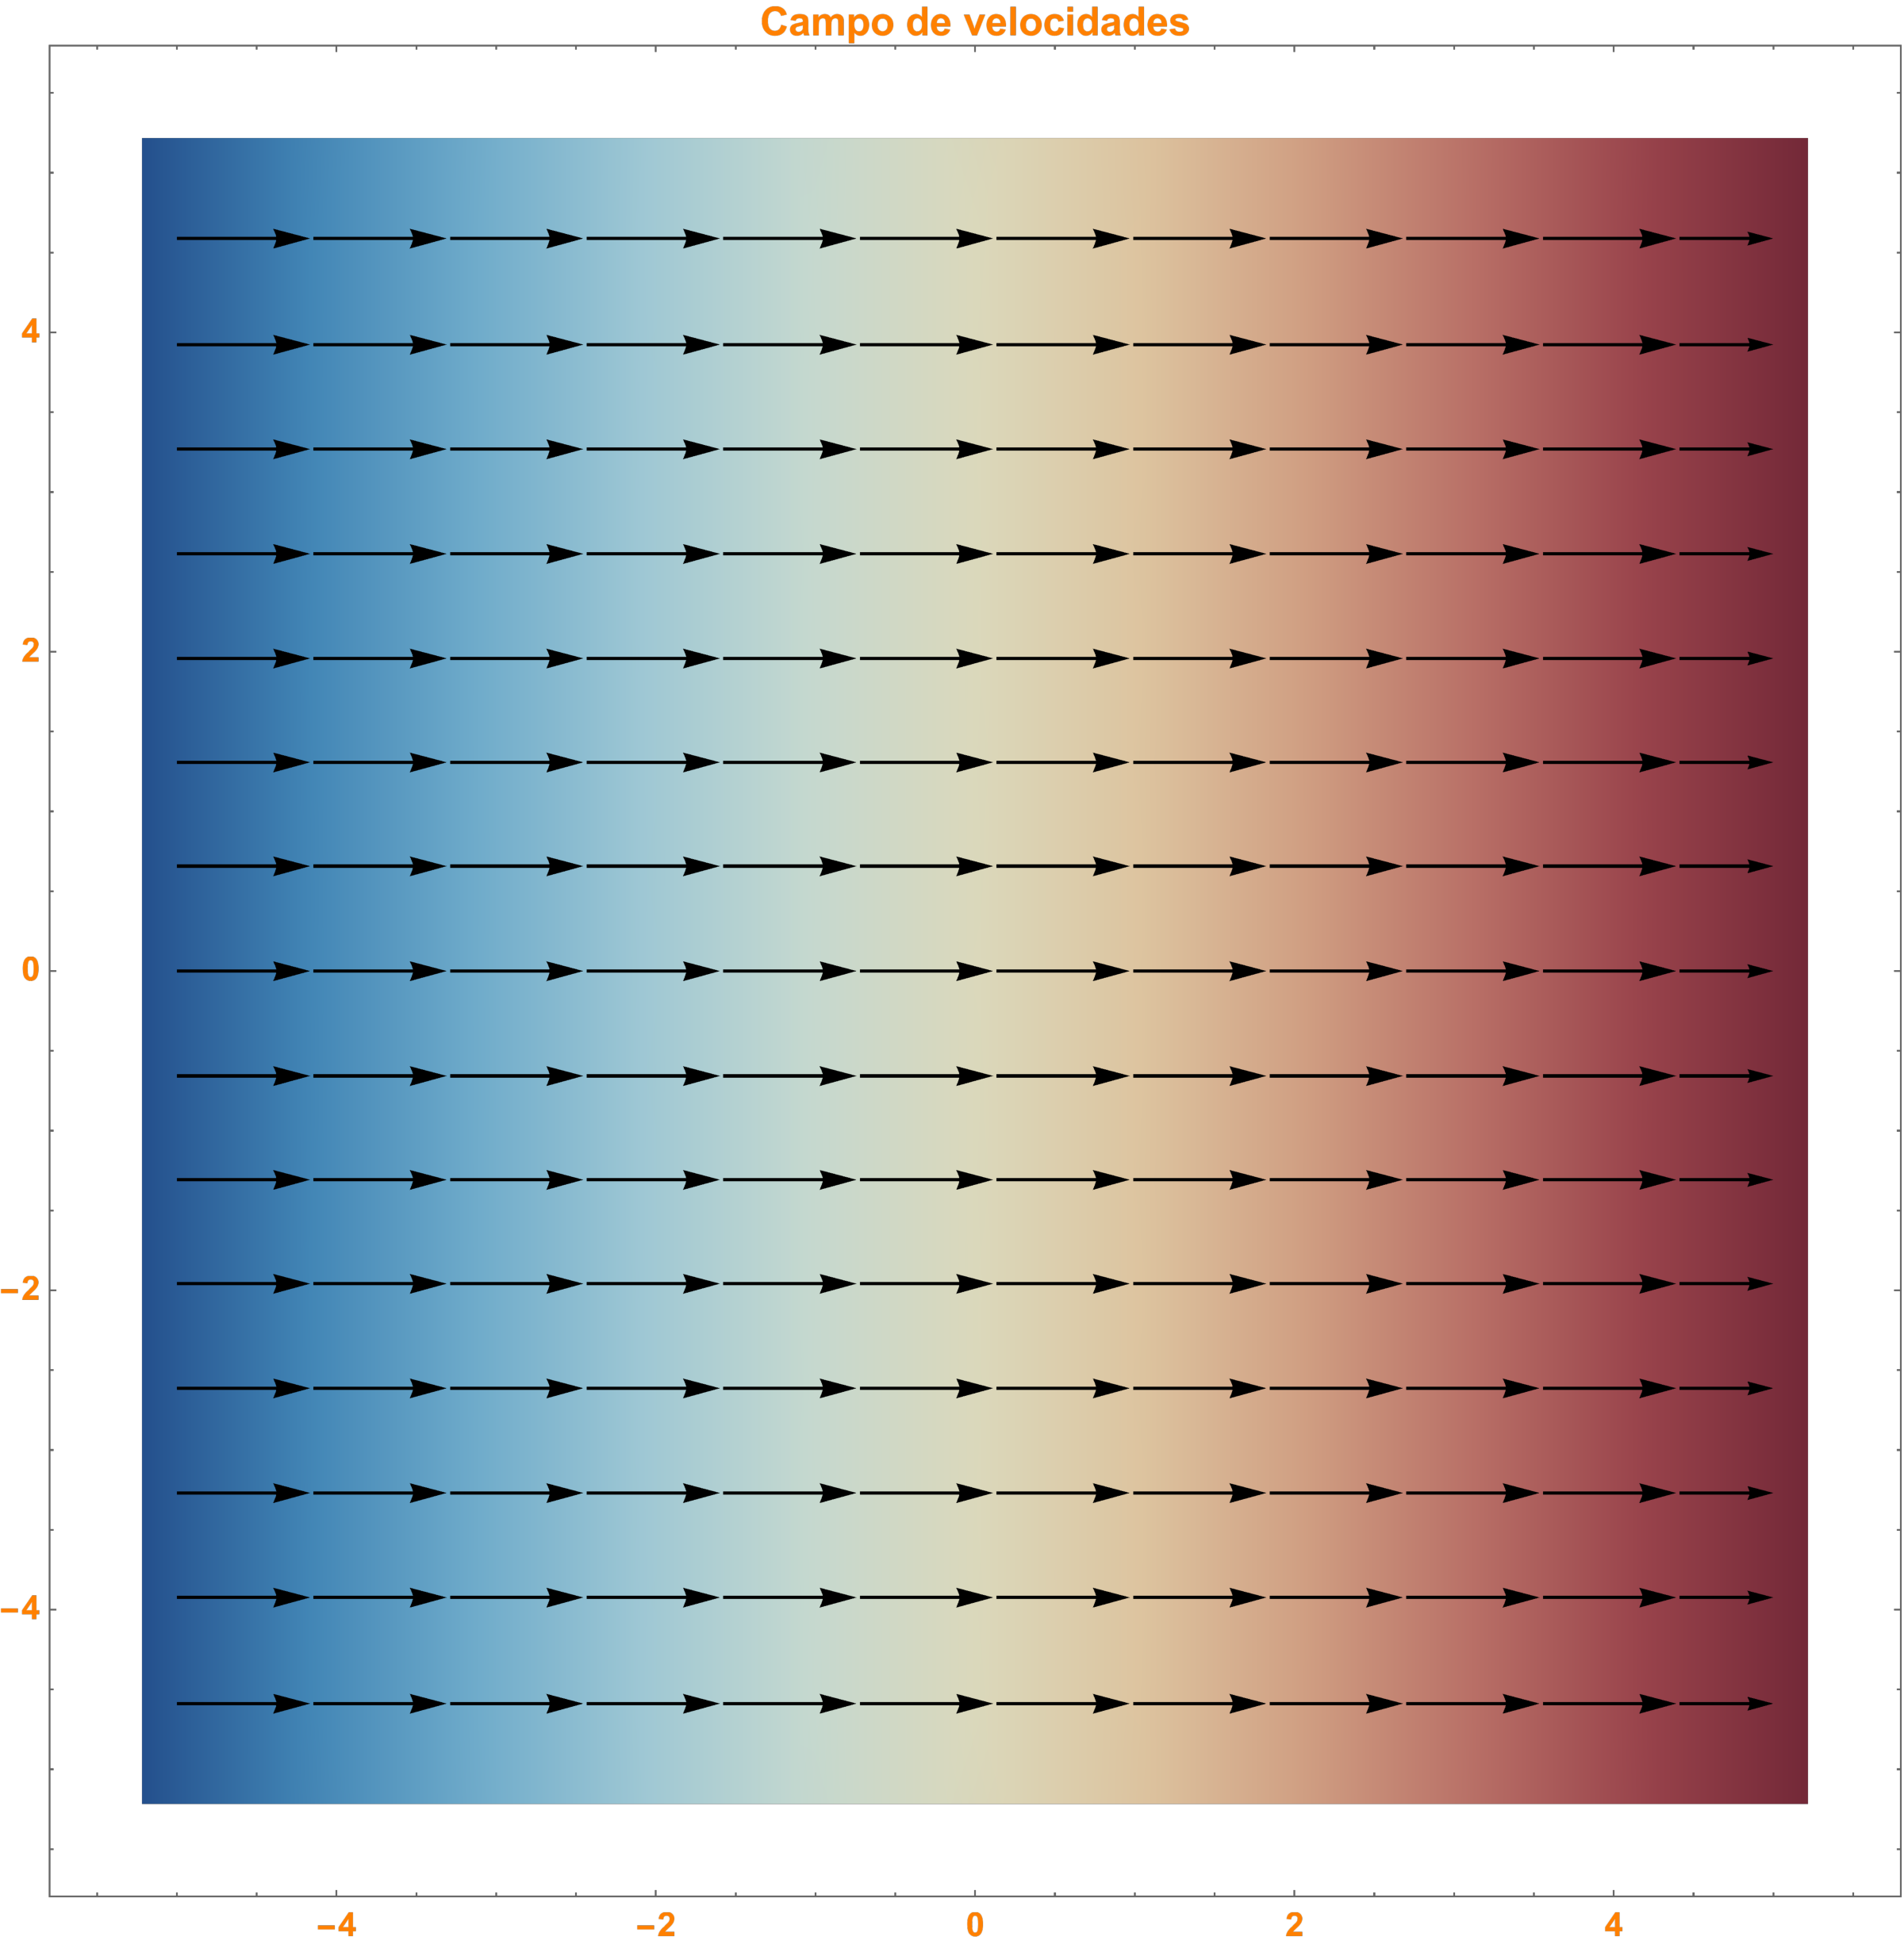
\includegraphics[width=0.5\linewidth]{vejercicio1.pdf}
%  \caption{El aburrido campo de velocidades (en el eje horizontal está $x_1$, en el vertical, es lo mismo, $x_2$ ó $x_3$). Los colores muestran el campo de temperatura.}
%  \label{gab}
%\end{figure}
%
%
%
%\textbf{c)}
%
%El campo de temperatura aumenta con la coordenada espacial $x_1$, con una funcionalidad simple $\Theta  = Ax_1$. Tenemos entonces:
%
%\begin{equation}
%\frac{D \Theta}{D t} = \overbrace{\frac{\partial \Theta}{\partial t}}^0 + \frac{\partial \Theta}{\partial x_i} \frac{\partial x_i}{\partial t} = \frac{\partial \Theta}{\partial x_i} \frac{\partial x_i}{\partial t} = A k 
%\end{equation}
%
%\noindent con lo cual podemos vislumrar que, si el campo de temperatura tiene una tasa de aumento $A$ respecto de la coordenada $x_1$ y las partículas viajan aumentando esa coordenada en el tiempo a una tasa (velocidad) $k$, entonces la temperatura de una partícula aumenta a una tasa $Ak$, lo cual no es desquiciado.
%
%\section*{Ejercicio 5}
%Considere el continuo cuyo campo de velocidad viene dado por:
%
%\begin{equation} \nonumber
%v_i=\dfrac{x_i}{1+t}
%\end{equation}
%\noindent Encuentre la ecuaci\'on de movimiento y el campo\footnote{Esta palabra está mal aquí, cuando hablamos de campo en general pensamos en una representación espacial, y lo que pide a continuación es la descripción material...} de aceleraci\'on en la descripci\'on material.
%
% ----------------------------------------------------------------------
% 
%Bueno, acá va prolijo. Recuerdo de notación:  Minúsculas, escalares. Mayúsculas, tensores (salvo coordenadas materiales). Negritas, vectores. 
%\vspace{1cm}
%a) Ecuaciones de movimiento:
%
%Como ya sabemos, las ecuaciones de movimiento son $x_i = f(\mathbf{X}, t)$
%
%La velocidad está en la descripción espacial, es decir,  $v_i(x_i, t)$. Concretamente:
%
%\begin{equation}\label{ev}
%v_i =\dfrac{x_i}{1+t}
%\end{equation}
%
%\noindent ojo que la ec. anterior no tiene como definición la definición de velocidad. La función $v_i(x_i, t)$ describe el cambio de velocidades de las partículas \textit{que pasan} por un punto fijo $x_i$ en un marco de referencia, y no el cambio en la posición respecto del tiempo de \textbf{una} partícula.
%
%Entonces, en la ec.(\ref{ev}) hacemos:
%
%\begin{equation}\label{eint}
%\dfrac{\partial x_i}{\partial t} =\dfrac{x_i}{1+t} \Rightarrow \int_{x_i = X_i}^{x_i} \dfrac{dx_i}{x_i} = \int_{t = 0}^{t} \dfrac{dt}{1+t}
%\end{equation}
%
%
%La solución a la ec.(\ref{eint}) queda:
%
%\begin{equation} \label{esol}
%ln\Big( \dfrac{x_i}{X_i} \Big) = ln(1+t) \Rightarrow x_i(X_i, t)  = X_i \; (1+t) + g(X_{j \neq i})
%\end{equation}
%
%\noindent si miramos la ec.(\ref{esol}) se nota que agregamos una función no especificada $g(X_j)$, para tener en cuenta que estamos integrando una ec. a derivadas parciales. La función $g(X_{j\neq i})$ es una función arbitraria de las coordenadas materiales...que no vamos a usar...pero que sería muy simple de calcular...¿cómo? Tarea pa las casas.
%
%El resultado que nos da para las ecs. de movimiento es entonces:
%
%\begin{eqnarray}
%\label{e51} x_1(X_1, t)  &= X_1 \; (1+t)& \\
%\label{e52} x_2(X_2, t)  &= X_2 \; (1+t)& \\
%\label{e53} x_3(X_3, t)  &= X_3 \; (1+t)& \
%\end{eqnarray}
%
%
%\textbf{b)} ...calcular la aceleración en la descripción material, es decir, la tasa de cambio temporal en las velocidades de cada partícula.
%
%Esto es, de la ecs.(\ref{e51}, \ref{e52}, \ref{e53}) hacemos:
%
%\begin{equation} \label{eacel}
%a_i(\mathbf{X}, t) = \dfrac{\partial^2 x_i(\mathbf{X}, t)}{\partial t^2}
%\end{equation}
%
%Lo que nos deja:
%
%\begin{equation}
%a_i = 0 \; \forall i= 1,2,3
%\end{equation}
%
%
%Entonces, las partículas no experimentan aceleración a pesar de que la velocidad en un punto del campo cambia en el tiempo.
%
%\line(1,0){100}
%
%\line(1,0){180}
%
%
%\section*{Consulta Ejercicio 6}
%Dado el campo de velocidad:
%
%\begin{equation}\label{ee6}
% v_1=-2x_2 \; \; \; v_2=2x_1
%\end{equation}
%\begin{itemize}
%\item[a)] Encuentre el campo de aceleraci\'on.
%\item[b)] Obtenga la expresi\'on de la linea de camino (``pathline'') del continuo. 
%\item[c)] Grafique el campo de aceleración en la descripción espacial.
%\end{itemize}
%
%%\line(1,0){100}
%\textbf{a)} Encontrar el campo de aceleración es simple, ya que contamos con la ecuación del Lai, 4$^{ta}$ ed. que dice:
%
%
%\begin{equation}\label{ealai}
%\mathbf{a} = \dfrac{\partial \mathbf{v}}{\partial t} + \nabla \mathbf{v} \; \mathbf{v}
%\end{equation}
%
%Podemos calcular, usando las ecs.(\ref{ee6}), las funciones que posee la expresión (\ref{ealai}), con lo que el primer término queda:
%
%\begin{equation}
%\dfrac{\partial \mathbf{v}}{\partial t} = \mathbf{0}
%\end{equation}
%
%\noindent es decir, la velocidad en un punto (descripción espacial) no cambia con el tiempo. Sólo depende de las coordenadas espaciales.
%
%El segundo término de la ec.(\ref{ealai}) queda:
%
%\begin{eqnarray}
%\nonumber
%\nabla \mathbf{v} \; \mathbf{v}  = &    
%\begin{pmatrix}
%\partial v_1 / \partial x_1 &  \partial v_1 / \partial x_2 & \partial v_1 / \partial x_3\\ 
%\partial v_2 / \partial x_1 &  \partial v_2 / \partial x_2 & \partial v_2 / \partial x_3\\ 
%\partial v_3 / \partial x_1 &  \partial v_3 / \partial x_2 & \partial v_3 / \partial x_3\\ 
%\end{pmatrix}
%\begin{pmatrix}
%v_1 \\
%v_2 \\
%v_3 \\
%\end{pmatrix}
%\Rightarrow & \\ 
%\nabla \mathbf{v} \; \mathbf{v}  = &  
%\begin{pmatrix}
%0 &  -2 & 0 \\ 
%2 &  0 & 0 \\ 
%0 &  0 & 0 \\ 
%\end{pmatrix}
%\begin{pmatrix}
%-2 x_2 \\
%2 x_1 \\
%0 \\
%\end{pmatrix}
%= & 
%\Big( -4x_1 \; \; -4x_2 \; \; 0 \Big)
%\end{eqnarray}
%
%\noindent juntando lo anterior, tenemos que la aceleración en la descripción espacial (el \textit{campo} de aceleración) es:
%
%\begin{equation} \label{e6ae}
%\mathbf{a}(x_1,x_2) = -4 x_1 \mathbf{e_1} - 4x_2 \, \mathbf{e_2}  
%\end{equation}
%
%\noindent una cosa interesante del campo de velocidades y el de aceleración, dado por la ec.(\ref{e6ae}) es que:
%
%
%\begin{equation}\nonumber
%\mathbf{v} \cdot \mathbf{a} = \Big(-2x_2\, \mathbf{e_1} + 2x_1 \, \mathbf{e_2} \Big) \cdot \Big(-4 x_1 \mathbf{e_1} - 4x_2 \, \mathbf{e_2}\Big) = \mathbf{0}
%\end{equation}
%
%\noindent lo anterior nos da una idea de movimiento circular, ¿no?, la aceleración perpendicular a la velocidad para cualquier tiempo y para cualquier coordenada...
%
%
%--------------------------------
%
%
%\textbf{b)} Encontrar la trayectoria o \textit{pathline}
%
%Las trayectorias son, simplemente...las trayectorias\footnote{El conjunto de puntos $x_1, x_2, x_3$ que conforman las posiciones de una partícula para cierto intervalo de tiempo.}, y están definidas por la ecuación de movimiento $\mathbf{x}(\mathbf{X}, t)$. Sin embargo, a veces es posible deshacerse del parámetro del tiempo, combinando las ecuaciones.
%
%A veces simple, otras no tanto, en este caso:
%
%
%\begin{eqnarray}
%\label{e61} v_1 = \dfrac{\partial x_1}{\partial t}  = -2 x_2  \\
%\label{e62}v_2 = \dfrac{\partial x_2}{\partial t} = 2 x_1 \
%\end{eqnarray}
%
%
%
%
%\noindent derivando respecto del tiempo las ecs. anteriores, tenemos:
%\begin{eqnarray}
%\label{e61s}\dfrac{\partial^2 x_1}{\partial t^2}  = -2 \dfrac{\partial x_2}{\partial t} = -4x_1 \\
%\label{e62s}\dfrac{\partial^2 x_2}{\partial t^2}  = 2 \dfrac{\partial x_1}{\partial t} = -4x_2 \\
%\end{eqnarray}
%
%\noindent las ecs.(\ref{e61s} y \ref{e62s}) ya están separadas (no tienen términos cruzados), y pueden integrarse dos veces para dar:
%
%\begin{eqnarray}
%\label{e61ss}x_1 = r\; cos(2t) \\
%\label{e62ss}x_2 = r\; sin(2t) \\
%\end{eqnarray}
%
%\noindent donde $r = \sqrt{X_1^2 + X_2^2}$ es la constante de integración de las ecs(\ref{e61s} y \ref{e62s}). Nos salteamos algunos pasos, pero si derivamos dos veces las ecs.(\ref{e61ss} y \ref{e62ss}), se puede ver que obtenemos las velocidades y las aceleraciones que calculamos. 
%
%Dicho lo anterior, queda saber que las ecs.(\ref{e61ss} y \ref{e62ss}) nos dicen explicitamente que esto que teníamos entre manos es un movimiento circular...de hecho, podemos sacar el pathline y deshacernos del tiempo, usando la identidad trigonométrica fundamental:
%
%\begin{equation}
%x_1^2 + x_2^2 = r^2 \equiv constante \label{e63sol}
%\end{equation}
%
%\noindent con todo este complicado proceso, tenemos el \textit{pathline} o \textit{trayectoria} de la partícula es un círculo cerrado.
%
%\line(1,0){100}
%
%\textbf{c)} Graficar el campo de aceleración es simple con Mathematica. No hay que perder de vista que un campo vectorial se grafica habitualmente con vectorcitos en una red definida de puntos. Lo podemos hacer con el comando:
%
%\begin{lstlisting}[language = Mathematica]
%StreamDensityPlot[{{-4 x, -4 y}, div[x, y]}, \{x, -5, 5}, \{y, -5, 5},
%ColorFunction -> "RedBlueTones", StreamStyle -> Black,  
% StreamPoints -> Medium, ImageSize -> Large]
%\end{lstlisting}
%
%
%\begin{figure}[h!]
%\begin{subfigure}{.50\textwidth}
%  \centering
% \title{Gráfico de Contorno de $\chi^2$}  
%  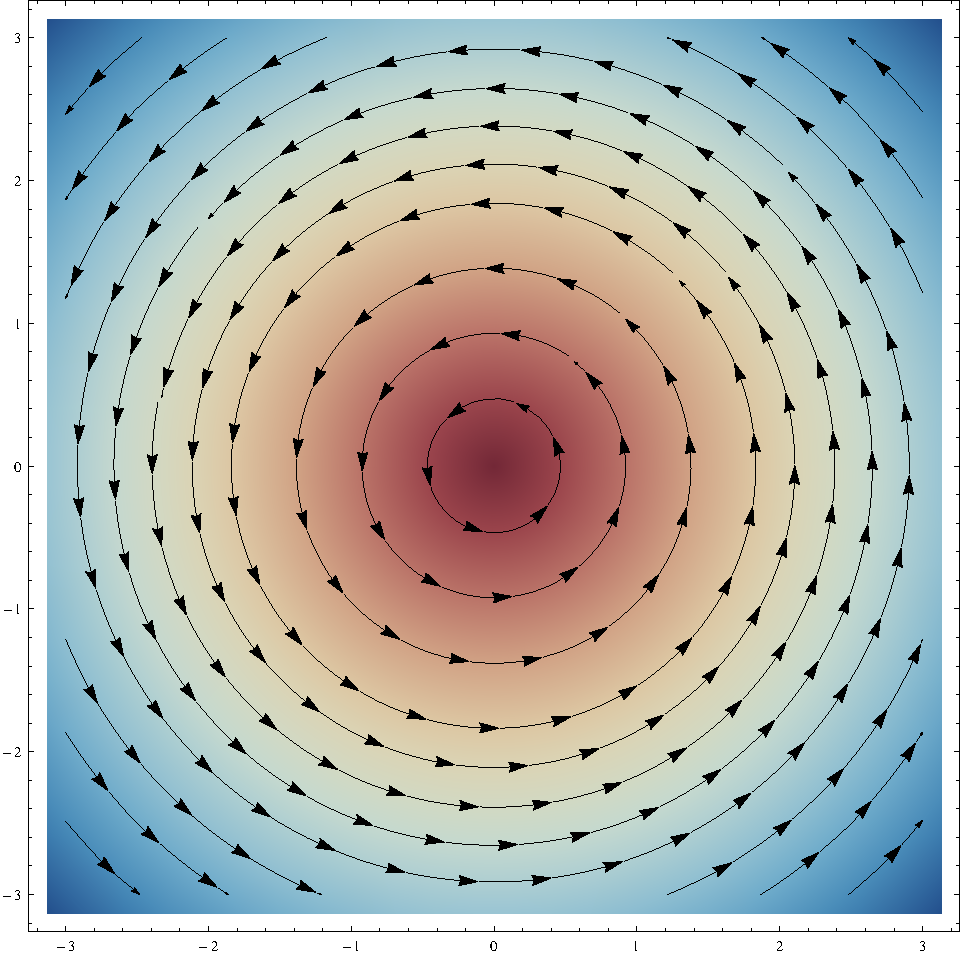
\includegraphics[width=1\linewidth]{vel6.pdf}
%  \caption{Velocidad, Descripción espacial.}
%  \label{gconto}
%\end{subfigure}%
%\begin{subfigure}{.50\textwidth}
%\title{} 
%  \centering
%   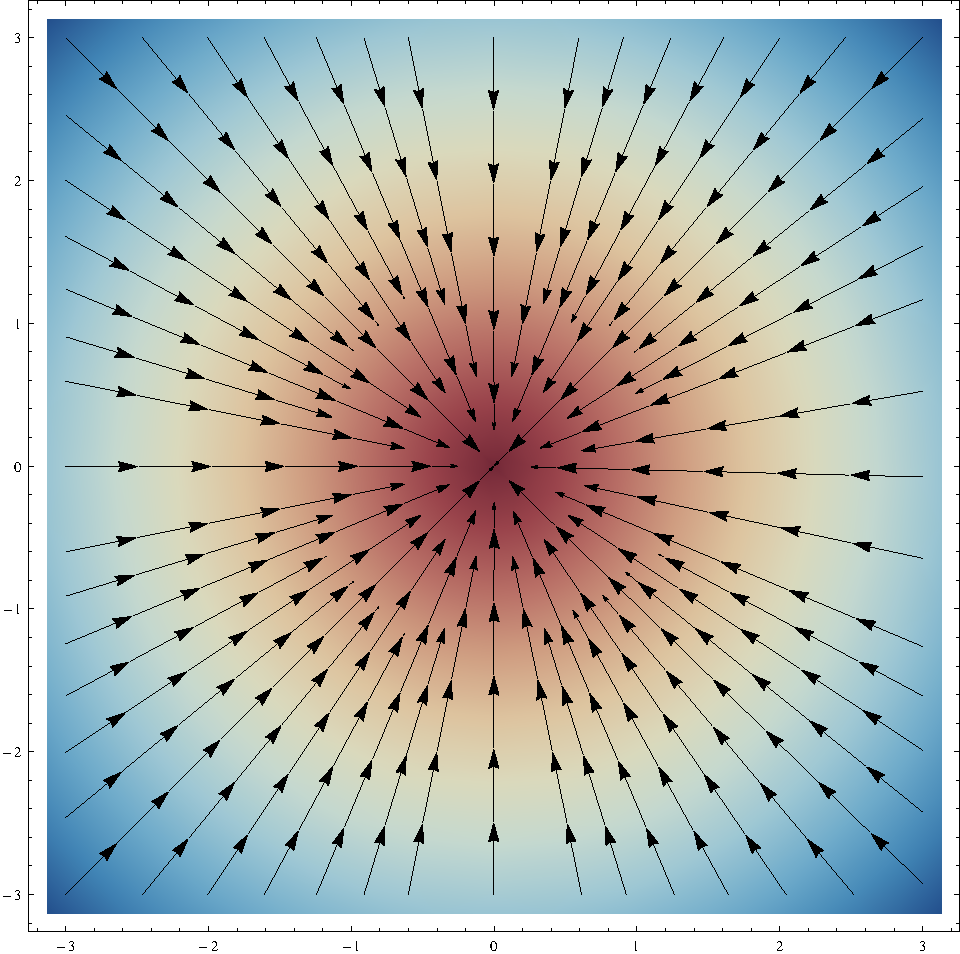
\includegraphics[width=1\linewidth]{acel6.pdf}
%  \caption{Campo de aceleración.}
%  \label{gtresd}
%\end{subfigure}
%\caption{Los colores representan la divergencia del campo  (y no se los pude sacar fácilmente!). Sin embargo se ve bonito...es importante notar que es de hecho un campo que se mueve de manera circular en torno a $\mathbf{x = \mathbf{0}}$.}
%\end{figure}
%
%Bueno, nos veremos el miércoles para cerrar este práctico y comenzar el nuevo. Buen fin de semana, disculpen por la demora.
%
%
%

\end{document}
